\section{Diagrams}

\subsection{Class Diagram}
This section details the changes made to the original class diagram.
\begin{figure}[h]
  \centering
  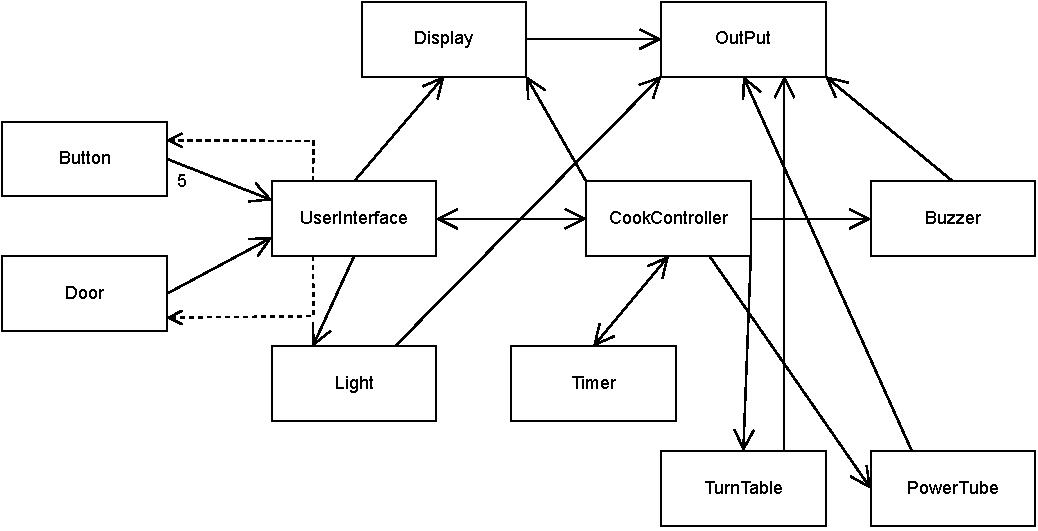
\includegraphics[scale=0.66]{02-Body/Image/ClassDiagram}
  \caption{Updated Class Diagram}%
  \label{fig:ClassDiagram}
\end{figure}
We have added two new classes. TurnTable and Buzzer.
The Buzzer has a uni directional association with the CookController class.
The TurnTable has a uni directional association with the CookControler and the Output class.
Lastly we added two more buttons to support the new features in the timer class.

\subsubsection{Short Description for Timer}
For the timer, we chose to make use of extra buttons to implement the adjust time features.
The buttons being a Increase Time Button and a Decrease time button. The user interface 
implements eventhandler for when these buttons are pushed. Classing the AdjustCookingTime
method in the CookController. Telling it to increase or decrease cooking time by 30 seconds.

The CookController itself calls an AdjustTime method in the timer class that increase or decrease
the time remaining by the requested amount.


\newpage

\subsection{STM Diagram UserInterface}
\begin{figure}[h]
  \centering
  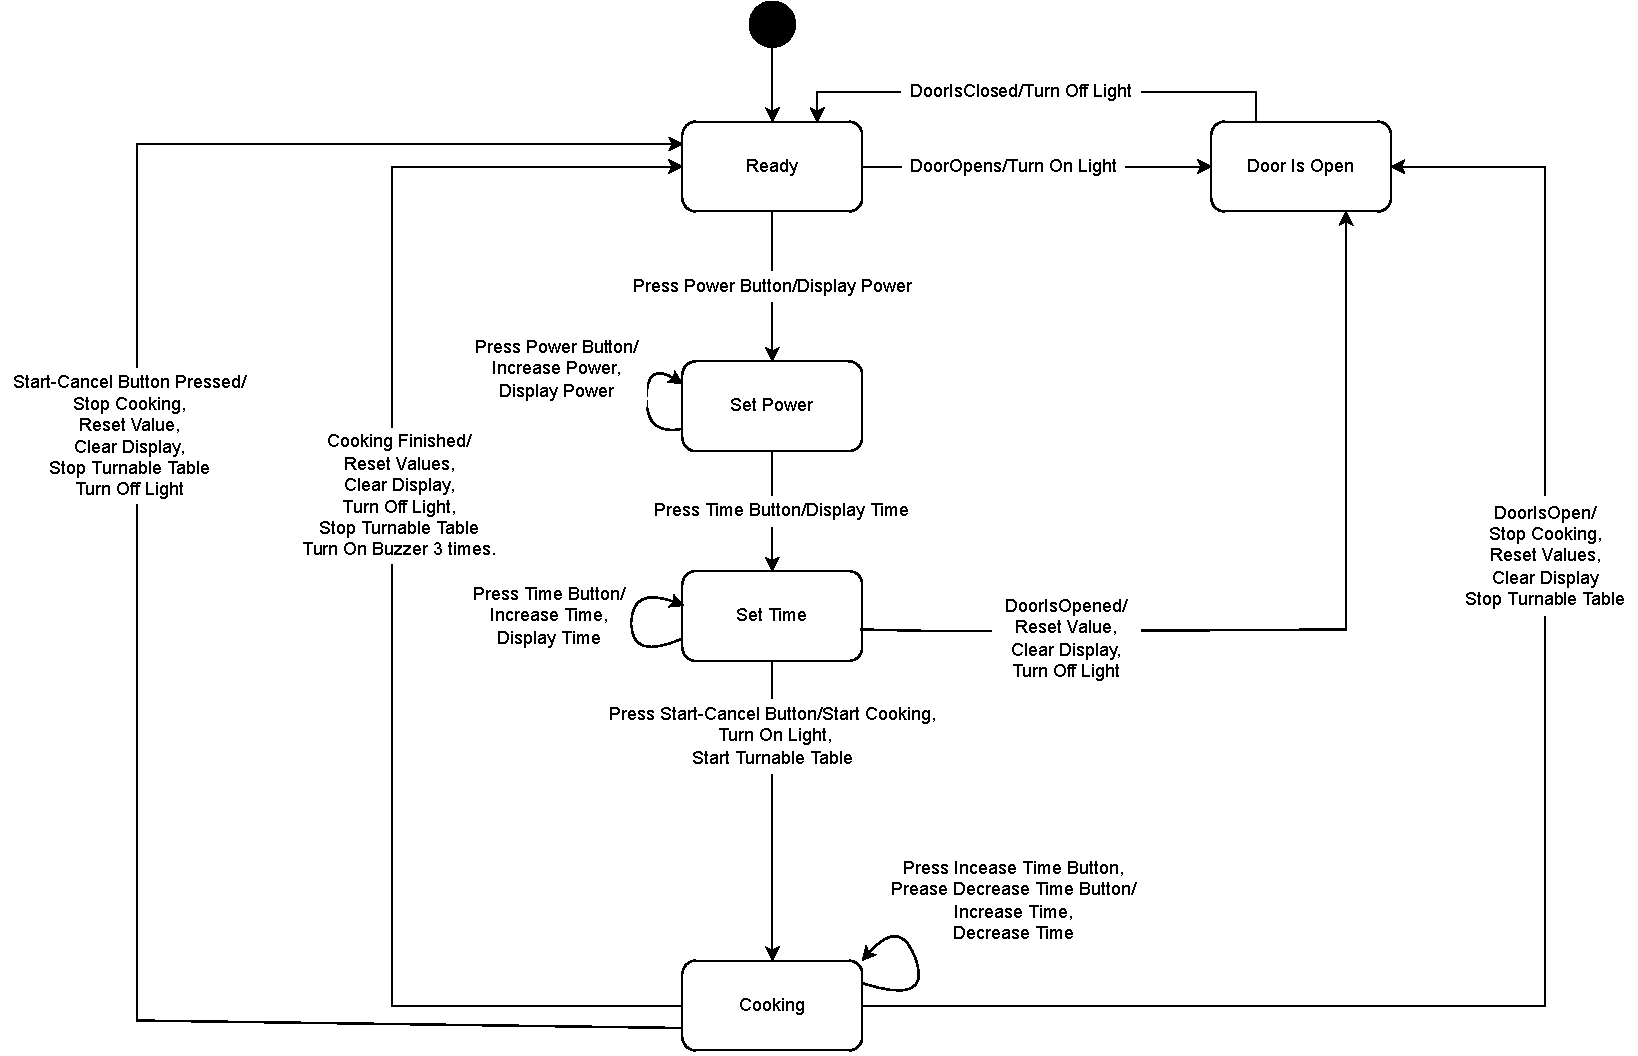
\includegraphics[scale=0.6]{02-Body/Image/STM_UserInterfacer.pdf}
  \caption{Updated STM diagram for UserInterface Class}%
  \label{fig:UserInterfaceSTM}
\end{figure}

\subsection{Sequence Diagram for Features}
\begin{figure}[h]
  \centering
  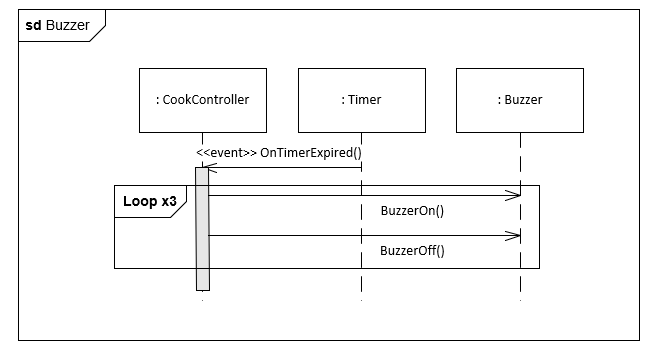
\includegraphics[scale=0.6]{02-Body/Image/BuzzerSEQ.PNG}
  \caption{Sequence diagram for CookControler interacting with Buzzer}%
  \label{fig:BuzzerSeq}
\end{figure}

\newpage
